\chapter{Métodos experimentales}

\section{Escritura de guías de onda}

\section{Montaje de excitación láser supercontinuo}

\newpage
\section{Montaje de modulación espacial de luz}

Para usar condiciones iniciales distintas a una gaussiana se hace necesario incorporar métodos de modulación espacial de luz. En esta tesis se utilizó una técnica conocida como 

\subsection{Etapa premodulación}
	El modulador espacial de luz utilizado es un HOLOEYE PLUTO-NIR SLM -  Reflective LCOS, cuya respuesta óptica ocurre con polarización paralela al plano de la mesa óptica. Se utiliza un retardador de media onda ($\lambda/2$) para que la polarización del la luz láser coincida con la de la respuesta del SLM. Posteriormente se magnifica y se colima el haz para que abarque todo el área de pixeles disponible.
\subsection{Etapa de modulación}

\subsection{Etapa de de-magnificación}
\subsection{Etapa de acoplamiento}
\subsection{Etapa de captura en cámara}

\subsection{Circuito óptico}
\begin{figure}[H]
	\centering
	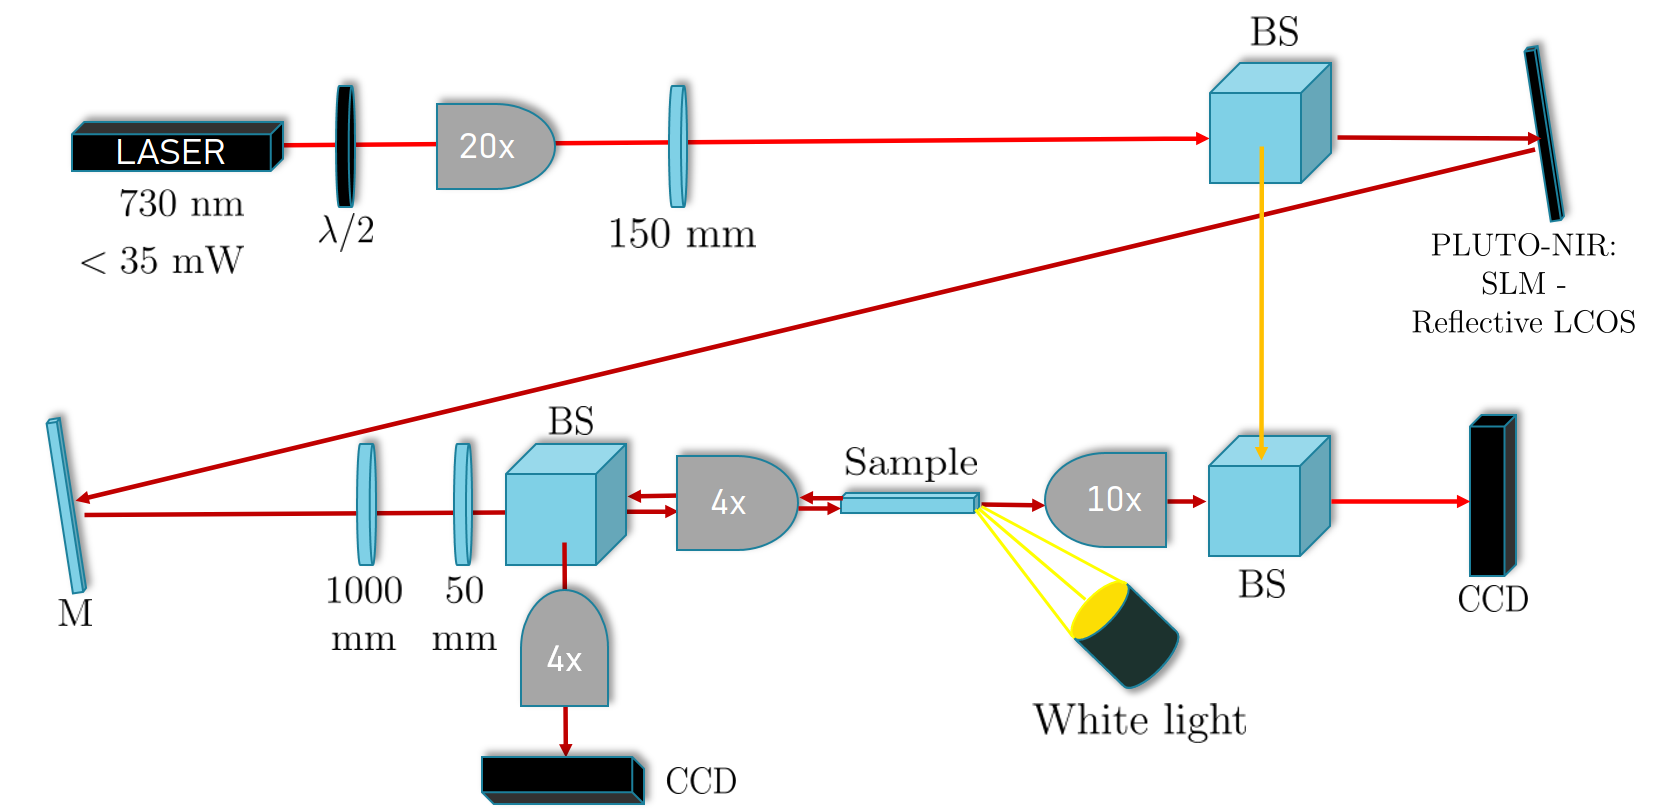
\includegraphics[width=\linewidth]{media/SLMsetup}
	\caption{Montaje SLM.}
\end{figure}
\subsection{Generación de hologramas}
\section{Análisis de imágenes}

